\documentclass[11pt,a4paper]{article}

\usepackage{graphicx}
\graphicspath{{images/}{report/images/}}

\title{Briscola Vision}
\author{Group members: \texttt{TODO}}
\date{\texttt{TODO}}

\begin{document}

\maketitle

\section{Introduction}

This project addresses the Briscola project.
Given a complete game as a folder of round videos, the system must infer the
cards played by both players, the leader, the briscola card, the winner and
points of each round, and the final game result. The provided ground-truth CSV
files are used to evaluate these predictions.

Our work focuses on comparing alternative computer-vision pipelines while
keeping game orchestration, Briscola rules, output, and evaluation shared.

\section{Shared architecture}

The visual method can change, while Briscola rules, scoring, video order, CSV
output, and evaluation stay the same. We keep these parts separate so that a
vision pipeline only produces evidence, while the shared game code calculates
the round outcomes and final result. In this way, every pipeline uses the same
game rules and can be compared fairly.

We analyse one round video at a time because it contains the information for
one trick. An \texttt{IRoundAnalyzer} reads a video and returns a
\texttt{RoundObservation}, while \texttt{GameRunner} orders the videos, gives
each round its number, and collects the observations. The fields in
\texttt{RoundObservation} are optional because a card can be covered, blurred,
or missed by the detector. Rather than forcing a guess, the system leaves that
value empty and calculates an outcome only when it knows both cards, the
leader, and the briscola. This stops a weak vision result from silently
changing the game score.

The briscola is handled by a separate \texttt{IBriscolaProvider} because it
belongs to the whole game, not to one round. Depending on the pipeline, it can
be found from one frame, from round candidates, or by voting across the game.
This choice does not affect the round analyzer, while the shared debugging and
evaluation make the different choices easy to compare.

\section{Vision pipelines}

\subsection{YOLO and local-feature pipeline}

\subsubsection{Overview}

This pipeline has two steps: a one-class YOLO oriented-bounding-box model first
finds physical cards, then local features identify each one by comparing it
with the 40 reference scans. We did not train YOLO to recognise 40 classes.
Instead, it only learns the shape of a card, while the reference scans handle
the card identity. This makes the detector and classifier easier to improve
separately.

\begin{figure}[h]
    \centering
    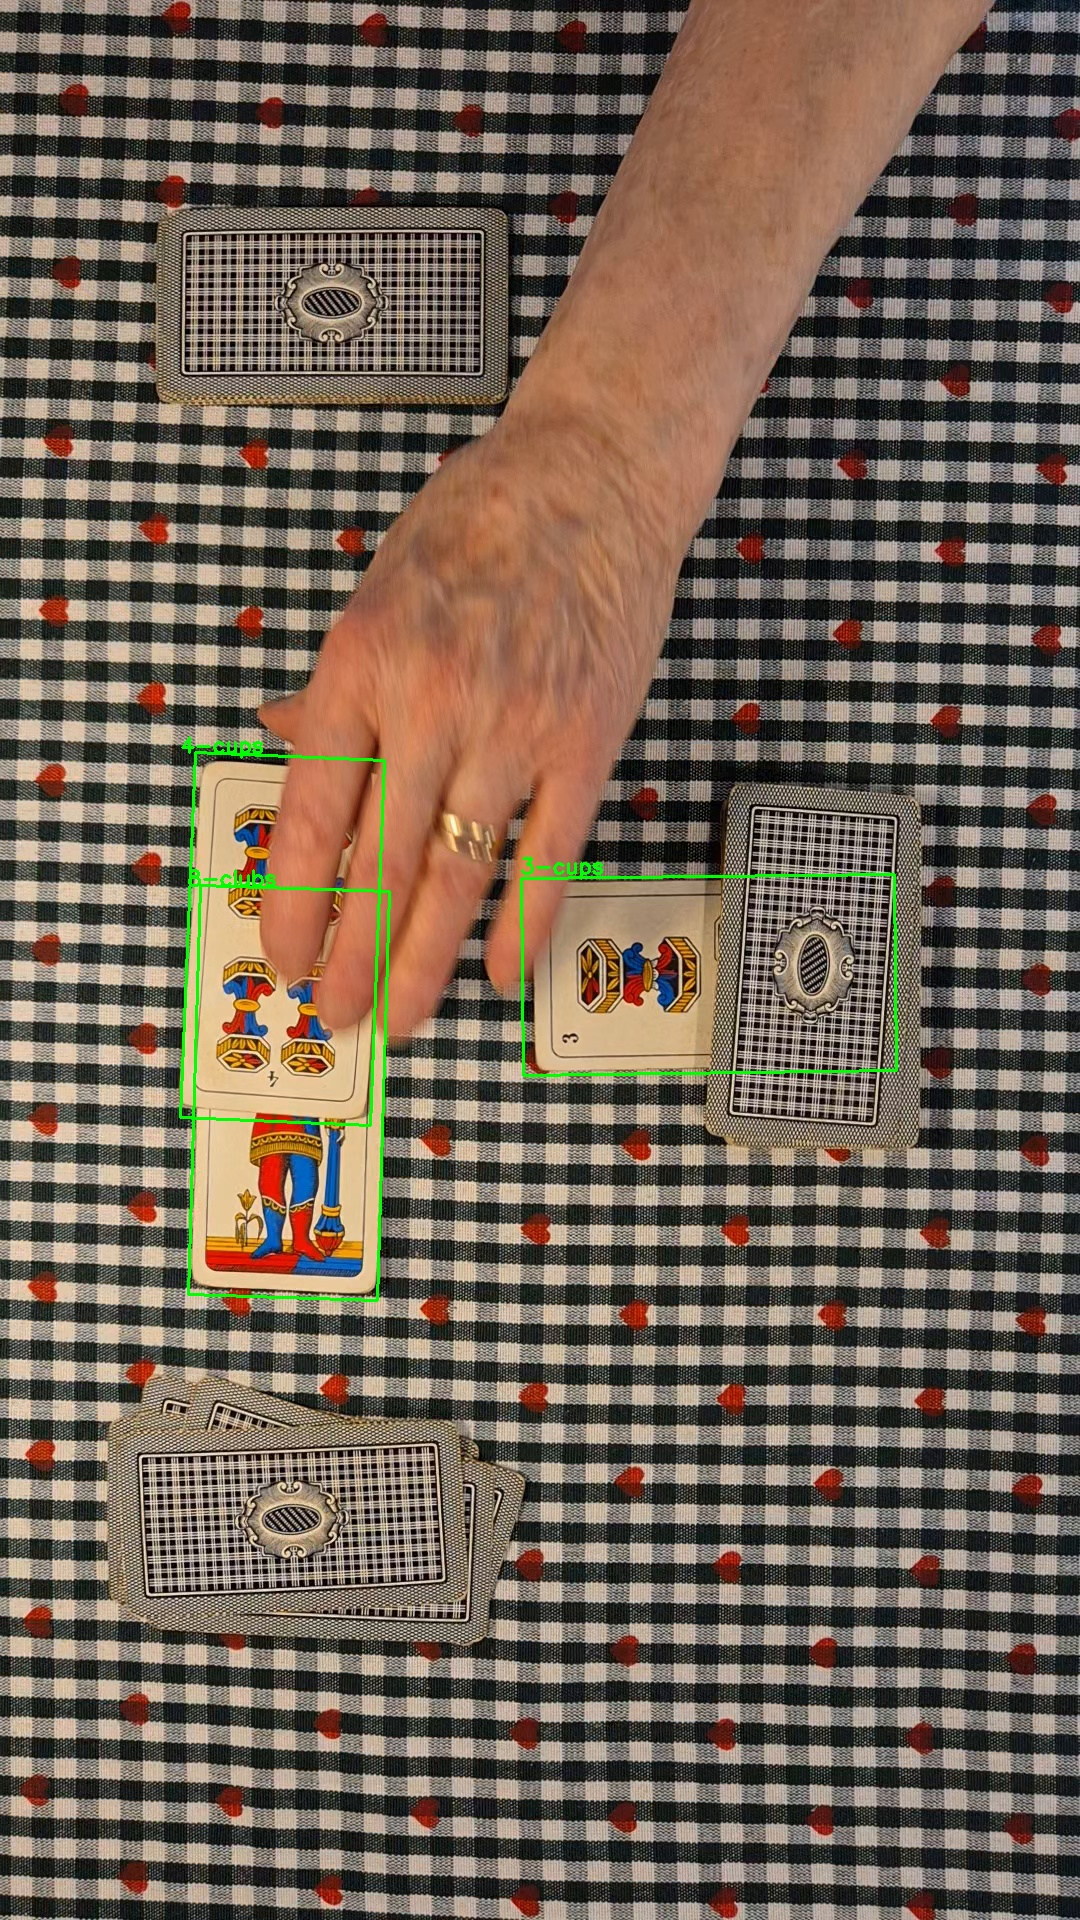
\includegraphics[width=0.42\linewidth]{yolo-pipeline.png}
    \caption{Debug output on a difficult frame. Even with a hand covering part
    of the cards, the pipeline detects and classifies the visible face-up cards.}
    \label{fig:yolo-orb-pipeline}
\end{figure}

\subsubsection{Detector training}

We fine-tuned a pretrained YOLO OBB model on a synthetic one-class dataset,
because we did not have enough labelled video frames to train directly on them.
Card scans let us generate many different scenes. Each image contains 1--6
face-up cards on a DTD texture background, with changes in position, size,
rotation, perspective, overlap, and edge cropping. We also add brightness and
contrast changes, blur, and noise. Some backgrounds are scaled down to include
fine checked textures like those in the real tablecloth.

Card backs are added as unlabelled distractors. Although they look like cards,
they cannot be used in the game, so they are not ground truth. Including them
helps the detector avoid treating every card-like object as a useful face-up
card.

We use oriented boxes instead of normal axis-aligned boxes because we need the
four corners for perspective rectification. A card needs at least 30\% of its
area visible to be labelled, but its label still covers the whole physical card
when part of it is hidden. This gives a stable shape for rectification when
cards overlap or are cropped.

\subsubsection{Card classification}

We warp each oriented box to the same shape as the reference scans, 581
$\times$ 315 pixels, and test both the crop and its 180-degree rotation so that
upside-down cards can still match. The reference keypoints and descriptors are
computed once when the application starts, then each crop is compared with all
40 references.

At first, we used SIFT, but it caused a clear problem with the coins suit. The
same coin symbol appears at different sizes and positions on several cards, so
SIFT could match a large coin on one card with a smaller coin on another one.
Since rectification already gives us the expected size and orientation, we do
not need SIFT's scale invariance. The final method therefore uses one-level ORB
with Hamming distance, which has no scale pyramid and is much faster.

We use OpenCV's brute-force matcher, Lowe's ratio test, and a 60-pixel spatial
mask. The mask accepts a pair only when the two features are in similar places
on the normalised crop and reference. Since local features alone do not know
the full card layout, this reduces wrong matches between repeated symbols. We
also use OpenCV's matcher instead of our own distance loop because it runs the
same brute-force search much faster.

\subsubsection{Temporal aggregation}

One frame is not enough to decide a round because a card can be missed,
misclassified, or almost fully covered. We first tried to use a frame with two
vertical player-card boxes, but this failed when the second card covered the
first one: the cards were seen at different times, but never together.

The final method groups vertical detections by their predicted card over the
whole round and chooses the two stable card classes that appear most often.
Their median vertical position gives North and South, while the class that
appears stably first gives the leader. In this way, the method uses evidence
from the full video instead of relying on a single good frame.

A frame with exactly one horizontal card gives one vote for the briscola, and
the most frequent candidate from all rounds becomes the game briscola. One
wrong detection or classification therefore cannot decide the game. This method
uses some assumptions about this dataset: the briscola is horizontal and always
visible, while player cards are vertical and stay in upper and lower areas.
These are not Briscola rules, and other analyzers do not need to use them.

\subsubsection{Current configuration and limitation}

The final configuration uses 0.60 detector confidence, one-level ORB with
5,000 keypoints, and the 60-pixel spatial mask. We kept the high number of
keypoints because it improved card recognition, even though it makes the
pipeline slow. Every crop and its rotated version are matched with all 40
references, so feature extraction, mask creation, and brute-force matching take
most of the time. The pipeline is not real-time, but real-time use is not the
goal of this project.

\subsection{Other pipelines}

\subsection{K-Means and Bag-of-Visual-Words pipeline}

\subsubsection{Overview}

This pipeline explores how far a fully classical, non-neural detector and
classifier can go on the same task. The goal was not to beat YOLO/local-features
on accuracy, but to map the boundary of a bag-of-visual-words classifier when
the card is lying on a checked tablecloth, often partially covered by another
card. The detector is a K-Means segmentation followed by a geometric filter; the
classifier is a BoW vocabulary built from SIFT descriptors of the 40 reference
scans. The pipeline is fully deterministic (k-means is seeded at 42) and
requires no training data, no GPU, and no learned model.

\subsubsection{Detector: K-Means plus local variance}

The detector has to solve one specific problem: the card face and the light
squares of the tablecloth have nearly the same colour, so a plain K-Means on
the raw frame merges them. The pipeline therefore applies, before any
clustering, a Gaussian blur whose kernel is larger than one checkerboard
period. When the kernel spans at least one full light/dark cycle, every output
pixel is an average of several light and dark squares, and the tablecloth
collapses to a mid-gray while the card face survives almost unchanged.

The blur alone is not enough when the kernel is not perfectly matched to the
pattern. A local variance map is therefore computed on the blurred grayscale
frame with two box filters ($\mathrm{Var} = E[I^2] - E[I]^2$). The card face,
being spatially uniform, has near-zero variance; the residual checkerboard has
high variance. A threshold on this map produces a \emph{uniform mask} that
removes the surviving fragments of the tablecloth before connected components
see them.

K-Means is then run on the blurred colour frame with $K=6$; the five largest
clusters are taken as the table-colour model, and the brightest foreground
cluster is taken as the card face. The binary mask of this cluster is
intersected with the uniform mask, closed with a $21\times21$ rectangular
kernel to seal the holes left by the printed figures and the suit symbols, and
its outer contour is flood-filled. Each resulting blob is scored on five
geometric properties (area, aspect ratio, extent, solidity, rectangularity);
the highest-scoring accepted blob is taken as the card. Both the axis-aligned
bounding box and the rotated \texttt{minAreaRect} are returned, together with
an already axis-aligned card crop and an expanded silhouette that other
pipelines can use for inhibition.

\subsubsection{Recognition: Bag of Visual Words}

A vocabulary of $K=800$ visual words is built by running k-means over SIFT
descriptors extracted from the 40 reference cards and their augmented
variants. Each card is represented by a histogram over the visual words, and
a query crop is matched to the reference with the smallest chi-square
distance.

Three choices were made after observing the failure modes of earlier versions.

\textbf{Augmentation geometry.} The first version simulated occlusion by
painting a black rectangle over a portion of the card. This produced a
training set whose geometry did not match the real crops: the real crop from
the detector contains only the visible portion of the card, with no black
cover. The training set was therefore changed to crop the card to a fraction
of its area (40\%--90\% visible, centered), which reproduces the actual
geometry of the detector's output. This change alone raised the played-card
accuracy from 47.5\% to 60\% on the first game.

\textbf{Vocabulary size.} Several values of $K$ were tested, from 40 to 800.
Small vocabularies collapsed distinct cards onto the same words; the sweet
spot on this dataset was $K=800$, where the vocabulary is large enough to
separate the 40 cards and their variants without overfitting.

\textbf{Colour extension.} An HSV histogram was appended to the BoW histogram,
on the assumption that colour would help distinguish Clubs from Coins, the two
suits with the most similar silhouette. The extension was implemented and
tested, but it degraded the overall accuracy instead of improving it. The
most likely reason is that by adding a second,
coarser colour channel drowned the discriminative signal in the noise of the
tablecloth colours. The colour extension was therefore removed, and the final
pipeline uses the BoW histogram alone.

\subsubsection{Pipeline integration}

\texttt{KMeansBriscolaProvider::find} scans up to 30 frames per round, calls
\texttt{findBBox} on each, and on the first successful detection classifies the
aligned crop. The provider implements \texttt{IBriscolaProvider}, so it can be
plugged into the existing \texttt{GameRunner} without changes to the rules or
the I/O.

The same BoW classifier can also replace the built-in template matcher inside
the movement-pattern analyzer, via the \texttt{--bow} flag. The scheduling
logic (motion detection, three-frame selection, leader inference) is reused
unchanged; only the recognition step is swapped. Because the frames selected
by the movement analyzer contain multiple cards (the briscola and the played
cards), \texttt{findBBox} is called with an exclusion mask that hides the
cards already identified, so the largest remaining blob is the card we are
looking for. The mask is the expanded bounding box returned by the previous
\texttt{findBBox} call, so no extra geometry is computed.

\subsubsection{Results and limitations}

The briscola card was recovered correctly on all four provided games. The
played-card classification is around 50\% across the four games.

The failure mode is systematic and intrinsic to the bag-of-words paradigm. A
card whose visible face shows fewer symbols than the real card (four denari
visible on a six-coins, five spade tips visible on a four-spades) is
misclassified toward the visually present rank, because the histogram loses
the descriptors of the covered symbols and the nearest reference becomes a
different card that happens to share the visible pattern. SIFT, which matches
descriptors locally and uses geometric verification, does not suffer from
this failure mode and is the recommended method when occlusion is expected.

\section{Results and discussion}

All pipelines are run on the same supplied games and evaluated against the
corresponding ground-truth CSV files. We report cards, leaders and winners,
briscola, final game results, and execution time.

\begin{table}[h]
    \centering
    {\small
    \setlength{\tabcolsep}{3pt}
    \begin{tabular}{lccccc}
            \hline
            Pipeline & Cards & Leader/winner & Briscola & Game result & Time \\
            \hline
            YOLO + ORB & 98.75\% & 100\% & 75\% & 100\% & 28--34 min/game \\
            Other pipeline & \texttt{TODO} & \texttt{TODO} & \texttt{TODO} & \texttt{TODO} & \texttt{TODO} \\
            \hline
        \end{tabular}\par}
    \caption{Results on the supplied games.}
    \label{tab:results}
\end{table}

Across the four games, the pipeline correctly predicted 158 of 160 player
cards, all 160 leader/winner fields, three of four briscola cards, and all 12
final-game-result fields. The only briscola error had the correct suit but the
wrong rank; it therefore did not affect any round winner, score, or final game
result.

% Discuss only observed errors and the relevant speed/accuracy trade-offs.

\section{Conclusion}

% Summarize the best-performing pipeline, its main limitation, and one concrete
% improvement that would be worth pursuing.

\end{document}
